% vim:set textwidth=100:
% vim:set fo+=t:

\documentclass[12pt]{article}

\usepackage{amsmath}
\usepackage[nofiglist,notablist]{endfloat}
\usepackage[usenames,dvipsnames]{color}
\usepackage{color}
\usepackage{authblk}
\usepackage{graphicx}
\usepackage{palatino}
\usepackage[activate={true,nocompatibility},final]{microtype}
\usepackage[super,sort&compress]{natbib}
\pagenumbering{arabic}
\parskip = 0.08in \parindent = 0.0in

% Custom macros for author comments
\newcommand{\Alberto}[1]{\color{ForestGreen}#1\normalcolor }
\newcommand{\Justin}[1]{\color{blue}#1\normalcolor}
\newcommand{\Arijit}[1]{\color{yellow}#1\normalcolor}
\newcommand{\Ken}[1]{\color{red}#1\normalcolor}

\author{Arijit~Roy}
\author{Justin~L.~MacCallum}
\author{Alberto~Perez}
\author{Ken~A.~Dill}
\affil{Laufer Center for Physical and Quantitative Biology\\
    Stony Brook University\\
    Stony Brook, NY 11794-5252.}

\title{Physics-based protein structure prediction and design using the confinement method}

\begin{document}

\maketitle

\begin{abstract}

The calculation of free energy differences is of central importance in the simulation of biochemical
systems.  The computation of the free energy difference between pairs of macromolecule with large
conformational change is particularly a difficult task and computationally expensive with existing
methods. In this work, an improved version of the confinement approach is used to calculate absolute
free energies of bio molecular systems. The method does not require a reaction coordinate or
transition path. It is fast to compute. We show that the method correctly picks out the state of
lowest free energy of a pair of structures having similar sequence but different fold. We also show
using models from CASP9 that the method picks out native-like structures from misfolded or decoys,
provided at least one good structure is in the input set.

\end{abstract}


\section{Introduction}

In computational structural biology there are numerous cases where free energy between well defined
states are necessary. Examples ranges from small to large conformational change of protein due to
ligand binding, change of pH etc. Free energy also play an important role in case of protein
folding. The ground breaking work of Christian B. Anfinsen and coworkers showed that the native
structures of small globular proteins have a unique, thermodynamically stable native structure with
their conformation at the global free energy minimum. Regardless of the starting point or unfolding
it by changing different condition most proteins will finally assume the same structure. It is very
important for proteins to achieve their native conformation since defects in protein folding may be
the molecular cause of a range of human genetic disorder. For example a misfolded protein known as
prion when enters any healthy organism it converts properly folded protein into misfolded one.
Thus, Free energy can also act as a scale to identify between the misfolded and the native state of
the protein. These observations further give free energy a special importance in structural biology.

However, the theoretical calculation of conformational free energy change become difficult if the
states of interest are very different. In such scenario timescale involved in such tranformation may
be beyond timescale of direct classical molecular dynamics simulation.  Generally, in order to
calculate free energy a pathway or reaction coordinate is created with the intermediate structures.
Method like umbrella sampling, thermodynamic integration along with classical MD can suffer from
overlap problem and require large computational effort. The idea of reaction coordinate became more
complicated in case of protein folding.  As free energy landscape of the protein folding is rough,
it can be trapped in a energy well during its visit in the conformational space. Even with the
advanced method like replica exchange molecular dynamics the three dimensional structure may be
trapped in a local minima for a considerable time. Due to various reasons it can also be misfolded
and trapped in a local energy minima. And one can mistakenly identify the misfolded state as the
native state (give the example of human pin1ww domain from Benout Roux and Klaus Schultan).

Calculation of free energy has been successfully attempted by a number of groups (give examples). In
recent years methods like Refrence system method, Decativated Morphing, Orthogonal Space Random
Work, Confinement Method have came out for calculation of free energy method. Some of the groups
relies on one of the great strength of free energy calculation, that it is a state function and thus
it is independent of path.

In this work we have applied the confinement method which was originally devoled by Tyka et. al. and
Cecchini et. al.  This method relies on a thermodynamic cycle where first, non-harmonic degrees of
freedom are removed by applying a series of restraint to the system. Then the free energy of the
remaining harmonic system is obtained using a normal mode calculation and combined with the
non-harmonic part to give the total absolute free energy.  Previously, this method was applied to
calculate the conformational free energy of a 16 amino acid residue peptide, known as BHP.  We have
first reproduced that known result. Then we have applied this method to larger proteins for the
first time. The free energy of conformation of pair of proteins with similar sequence but completely
different fold was calculated. Encouraged by the result, we applied the method of different targets
of CASP9 competition.

%of protein can be obtained to atomic resolution by X-ray crystallography or NMR. Unfortunately, the
%sheer amount of time and economic investment for structure determination cannot keep up with the
%rate at which proteins of unknown structure are sequenced. Therefore, computational models can be a
%good way to bridge the increasing gap between sequence and structure. In this respect CASP
%(Critical Assessment of Structure Prediction) has played a crucial role which is a community wide
%experiments for the protein structure prediction.



\section{Results and Discussion}

\subsection{The confinement method produces correct results in control experiments}

As a first step, we performed several control experiments to verify that our implementation of the
confinement method produces results compatible with previous calculations reported in the
literature.

The method has previously been applied to a 16 amino acid residue $\beta$-hairpin from
protein G, known as BHP[ref]. We calculated the free energy difference between two different
conformations of the peptide: (1) the native conformation, called bhp1, with a two-stranded
$\beta$-sheet; and (2) a conformation, called bhp3, which has a three-stranded $\beta$-sheet.
Analysis of long (4 $\mu$s) equilibrium simulations[ref] shows that bhp1 is the more favorable
configuration by 1.8 kcal/mol. Using the confinement method, we obtain a value 1.7 kcal/mol, which
is in good agreement with the equilibrium simulations and with previous calculations using the
confinement method[ref] (see Supporting Information for further details).

\Justin{Arijit, Al: did we do any other control experiments on small peptides that we should report
here?}

Previous applications of the confiment method have focused on relatively short peptides, up to X
residues in length \Justin{Arijit: fill in X}. In this work we apply the confinement method to
larger proteins. One of the  applications we explore in the present work is the re-scoring, or
metaprediction, of structures submitted during the Critical Assessment of Structure Prediction
(CASP) experiment (described in detail later). We computed the relative free energies of predictions
submitted during CASP9 and 10, with the expectation that the most native-like prediction will have
the lowest free energy. As a control, for several targets we also calculated the relative free
energy of the experimental structure (once it was available from the PDB). As
Table~\ref{table:casp_control} shows, in X of Y cases, the confinement method correctly assigns a
lower free energy to the experimentally determined structure than to any of the decoys. Although
differentiating between experimentally determined structures and computer generated predictions is
not a stringent test of a scoring method---for example, examining the residue-residue packing can
easily distinguish between the two [ref Rosetta Holes]---the results none the less serve as a useful
"sanity check".

\begin{table}
\label{table:casp_control}

\begin{center}
\begin{tabular}{l l l}\hline
    CASP Target  & PDB Identifier & $\Delta\Delta G_{native \to best decoy}$ (kcal/mol) \\ \hline
\end{tabular}
\end{center}

\caption{The confinement method assigns a more favorable free energy to the experimentally
determined structure than to computer-generated predictions. For each target, we examined as many as
five predictions submitted by CASP participants. Positive $\Delta\Delta G$ values indicate that the
experimental structure is predicted to be more favorable than any of the decoys.}

\end{table}


\subsection{The confinement method correctly predicts the structural preferences of chameleon
sequences}

In general, proteins with similar sequences tend to have similar structures. This idea is the basis
of comparative modeling and fold recognition in protein structure prediction. There are, however,
examples---often referred to as chameleon sequences---of proteins with similar sequences that have
remarkably different structures. Orban and co-workers have designed a series of 56-residue proteins
(based on Protein G) that adopt one of two different folds depending on small changes in sequence
(see Figure~\ref{fig:orban}). Sequences that adopt a mixed alpha/beta structure similar to Protein G
are denoted as ``GB'', while sequences that form a three-helix bundle are denoted as ``GA''. One
pair of sequences (GA88/GB88) are 88 percent identical and differ in seven positions. Another pair
(GA95/GA95) are 95 percent identical and differ in three positions. The last pair (GA98/GB98) differ
only in a single tyrosine to alanine mutation.

The fact such small changes in sequence can lead to such dramatic changes in structure is rather
remarkable. Accurately predicting the structural preferences of these structures presents a serious
challenge for computational methods [ref].

We initially approached this problem by making a model of each sequence with the same backbone
structure as its partner chameleon sequence. For example, we took the sequence of GA88 and built a
model with the same overall structure as GB88. We then used the confinement method to assess the
free energy difference between the experimentally determined structure of GA88 and the model (with
the GA88 sequence and the GB88 structure). The confinement method was able to predict the
conformational preferences correctly for all six sequences (data not shown). There is, however, a
serious problem with this analysis: we are comparing an experimentally determined structure with a
computer generated model. It might be possible that we were able to make correct predictions simply
because artefacts of our modeling procedure always lead to the model having a higher free energy
than the experimental structure.

To avoid this potential problem, we instead computed the relative free energy two different
structural models for each sequence. One model is based on the GA structure and the other on the GB
structure (see Supporting Information for details on the modeling procedure). This is a much more
realistic test of the confinement method's ability to accurately calculate relative free energies.

The results of these calculations are presented in Figure~\ref{fig:orban}. The confinement method
identifies the correct structure for all six sequences. The free energy differences range from
around 2.9 to 5.7 kcal/mol, which is consistent with small changes in sequences and with estimates
made by Orban and co-workers [ref].

\begin{figure}
\label{fig:orban}

\caption{The confinement method correctly predicts the structural preferences of six chameleon
sequences. (A) The six sequences used in this study. (B) Each sequence adopts either a Protein
G-like fold (denoted GB) or a three-helix bundle fold (denoted GA). The relative free energies of
the two folds are reported for each sequence.}

\Justin{Arijit: we need to make this figure, which we've discussed before and move the data from the
following table into the figure.}
\end{figure}

%\begin{table}
%\caption{The confinement method correctly reproduces the structural preferences of a series of
%designed peptides. Each sequence adopts either a Protein G-like fold ($4 \beta + \alpha$) or forms a
%helix bundle ($3 \alpha$).}
%\label{table:orban}
%\begin{center}
%\begin{tabular}{l l l}\hline
%Changes in & $\Delta G$ (kcal/mol)    & $\Delta G$ (kcal/mol)     \\
 %Sequences & ($3 \alpha$ fold)        & ($4 \beta + \alpha$ fold) \\ \hline
%GA95       & $0.000$                  & $2.901 \pm 0.475$         \\
%GB95       & $4.365 \pm 0.460$        & $0.000$                   \\
%GA88       & $0.000$                  & $ 3.941 \pm 0.517$        \\
%GB88       & $5.576 \pm 0.464$        & $0.000$                   \\
%GA98       & \Justin{Arijit: fill in} &                           \\ \hline
%GB98       &                          &                           \\ \hline
%\end{tabular}
%\end{center}
%\end{table}


\subsection{The confinement method correctly identifies the most native-like predictions from a
subset of CASP predictions}
\Alberto{Arijit: we need a global table of success, rather than individual tables. The simplest form
    would have 3 columns: name of the PDB, number of structures tested, percent of success of
    picking 1st model}
\Alberto{Arijit: CASP notation should not be used (T????) instead, pdb code should be used}

This method is particularly well suited for events such as CASP (critical assessment of structure
prediction). CASP is a blind test world wide competition in which different groups apply their
methods to predict the 3D structure of proteins given their sequence. This is done with a strict 3
week limit on each target (3 day for servers) and each group is allowed to submit 5 possible
structures (ranked from better to worst). In our role as assessors during the CASP8 and CASP9 [CITE]
competition we observed no correlation at all between the ordering of structures submited by the
groups and the real ranking compared to an experimental model. The consequences of this go beyond
those five structures; the deeper meaning is that groups producing ensembles of structures are
generating structures that are better than the ones they submit, but they do not know about it. In
fact, when querrying different groups after the results were known, most groups agree that this is
the case. Beryond the CASP problem, this reflects on the modelers ability to correctly rank order
models in many different environments, from structures for drug design leads to designing more
stable proteins or peptide mimetics such as peptoids. One of the main culprits of this lack of
accuracy is the fact that ranking is often done via a potential energy function, which in many cases
lacks an entropy component. Other initiatives including knowledge based potentials do use some sort
of free energy to rank order, but its accuracy is not enough. Our method provides a physics based
solution to this problem. We have tried two experiments centered on CASP. First we tried to rank
order some structures from the previous CASP9 experiment. Our second test was to participate as a
metapredictor group in CASP10. In both methods, our ranking is determined as a free energy measure,
and it is compared with the ranking given by a geometrical comparison between native and submitted
models called GDT\_TS (Global distance test score [CITE, look in CASP9 refinement paper for cite
21]). GDT\_TS represent the average percentage of residues that are in close proximity in two
structures optimally superimposed using four different distance cutoffs (1, 2, 4 and 8 Å).

We have chosen the inital models on which to test the methods based on server groups that have
traditionally done good in past CASP events. There is a high correlation between the structures that
are chosen for this method and its predictive accuracy. In particular, when GDT\_TS scores are below
50, it is difficult for us to say anything about the models. Our approach is simple, with every
subset of structures we choose, we use the confinement method in a pairwise procedure, and then rank
the structures. Note that we do not need to make comparisons to native in order to rank order.

\Subsubsection{CASP9}
Can we distinguish between native and models? Identifying the native state from a set of models is a very easy test, that most metapredictors
already handle correctly, but it is also a first proof of principle. We exemplify this with
T0660\Alberto{Arijit:PDB code please, here can you complete the text in subsection T0560 or added it here
    directly?} by selecting the native state and comparing it to two models from the "Splicer"
server. Here, the main difference between the two models is the orientation of the ... As expected,
the native state is identified correctly, and the two other models is correctly identified. Our next test was to see if we could rank order within a given server's predictions. We chose
T0559 \Alberto{Arijit: change to PDB code, say CASP code T0559} and the BAKER-ROSETTASERVER. We
initlally checked similarity between the models and discarded two of them from the analysis on the
basis of being too similar to some of the other models. For the remaining structures, we correctly
ranked order the results as seen from Table~\protect\ref{tab:T0559}. This was a relatively easy test
as the differences in GDT\_TS score are fairly large. Therefore, our next test was between models
from the best submissions of different groups (range of GDT\_TS
from 96.23 to 80.66). Again, our method was able to correctly order the results
(Table~\protect\ref{tab:T0538}). \Alberto{I don't like so many small tables. Have to find out a way
    to combine into something bigger, so can check this whole paragraph in one table or figure.}
There are however some instances where the method can fail, specially when close GDT scores are
given. This is the case in T605, Table~\protect\ref{tab:T0605}, where the first model from the BAKER
group is correctly identified, put the 2nd and 3rd are given in inverse order. \Alberto{Airjit:
    Reasons for this???}

What can we say about low resolution models?
We mentioned earlier that our predictive abilities are greatly decreased with low model qualities.
We performed such a test with T0531, in which we compared the crystal structure to five models from
the MUFOLD server. Looking at table ~\protect\ref{tab:T0531} shows: 1.) native is correctly
identified as expected and 2.) Surprisingly there is a high level of correlation between the GDT
ranking and the free energy ranking, only two structures whith GDT\_TS < 30Å are ordered
incorrectly. It is worth to note that models 2 and 3 have the same GDT and very different free
energies, meaning that the actual ordering could change a lot [Cite FlexE].

\Subsubsection{CASP10}
We participated in CASP10 as a metapredictor group. Given the tigh schedule of the CASP competition,
we only attempted proteins under 100 residues in length. Our main problem during this part of the
competition was that proteins were trimmed from the actual calculation.
\Alberto{Justin,Arijit: Probably should not comment on metapredicting since we were not able to do
    good due to the trimming factor. Instead, we should move forward with Justin's idea of using
    structures that other meta predictors did badly at. What stage is that in?}

%The GDTTS value of a model is determined as follows. A large sample of possible structure
%superpositions of the model on the corresponding experimental structure is generated by superposing
%all sets of three, five, and seven consecutive C$\alpha$ atoms along the backbone (each peptide
%segment provides one superposition). Each of these initial superpositions is iteratively extended,
%including all residue pairs under a specified threshold in the next iteration, and continuing until
%there is no change in included residues. The procedure is carried out using thresholds of 1, 2, 4,
%and 8 $\AA$, and the final superposition that includes the maximum number of residues is selected
%for each threshold.

\Alberto{This subsections have to go. I'm momentarily leaving them on so you can complete the text
    with number of residues and maybe experimental origin. I would put the number of residues in the
    tables}
\subsubsection{T0559}

The native structure is a  67 residue NMR solved structure. We first reviewed all the five models
submitted by the group "BAKER-ROSETTASERVER", which was the best predictor group for this particular
target.  Among them we choose only the three structures, model 1, 3 and 5 to calculate the free
energy and subsequently identify the most stable structure among them. The rest of the two
structures are close to either of the selected structure and thus they are ommited from our
calculation. According to the GDT\_TS score, the model 1 was picked up correctly from the set of
structure generated . However, the order of model 3 and 5 was not correct as can be seen from the
Table 1. It will be interesting to know whether confinement method can order the strcutures in terms
of free energy scale. The result is presented in Table~\protect\ref{tab:T0559}.


\subsubsection{T0560}

Target T0560 is a 74 amino acid residue target from CASP9. However residues 3-66 were kept for final
result.  For this target we have compared the free energy of the model 2 and model 4 submitted by
the group "Splicer" along with the crystal structure.  The main difference between the model 2 and 4
is the orientation of the ....  The final result is presented in Table~\protect\ref{tab:T0560}.

\subsubsection{T0538}

Target T0538 was a 54 residue target. The native structure was generated using NMR. The best model
that is closest to the native structure was generated by the group PconsR. However, their model 3
was better than their model 1. This structure was quite close to the NMR structure and had GDT\_TS
value of 96.23. We have calculated the free energy between this structure and the best structure
submitted by the group "Shell", "FOLDIT" and "BAKER-ROSETTASERVER". The calculated free energy value
is presented in Table~\protect\ref{tab:T0538}.

\subsubsection{T0540}
\Alberto{Arijit: between T0560 and T0540, which one is better? I would keep only one of them, and my
    preference is T0560, we are showing the same test}

Target T0540 was a 90 residue target. We have taken the best models from the group "LTB" which was
the best performing group for this target and also from the group Mufold and calculated the free
energy difference between these models with that of the native crystal structure.  As expected, the
crystal structure has the lowest free energy value, followed by Model 1 with GDT\_TS score of
$69.72$ and model 2 with GDT\_TS value of $53.789$. The final result is presented in
Table~\protect\ref{tab:T0540}.


\subsubsection{T0531}

This is a 65 amino acid residue target with residues 6-63 were kept for final analysis. We have
calculated the free energy difference between all the five models submitted by the group
"MUFOLD-MD", which was one of the best performed group for this target.  The result is presented in
Table~\protect\ref{tab:T0531}



\subsubsection{T0605}

This is a 72 amino acid residue protein but for the final calculation only the residues 18-66 amino acids were kept for the final analysis.

The best performing group was "Baker" for this target. We have carried out our calculation with the model first, second and fifth for the
final calculation. The rest two model had closer GDT\_TS value compared to the previously mentioned models and thus they were omitted from
furthe calculation. The result is presented in Table~\protect\ref{tab:T0605}. (This is a case where we can demand the confinement
method is better than GDT\_TS).


\begin{figure}
\begin{center}
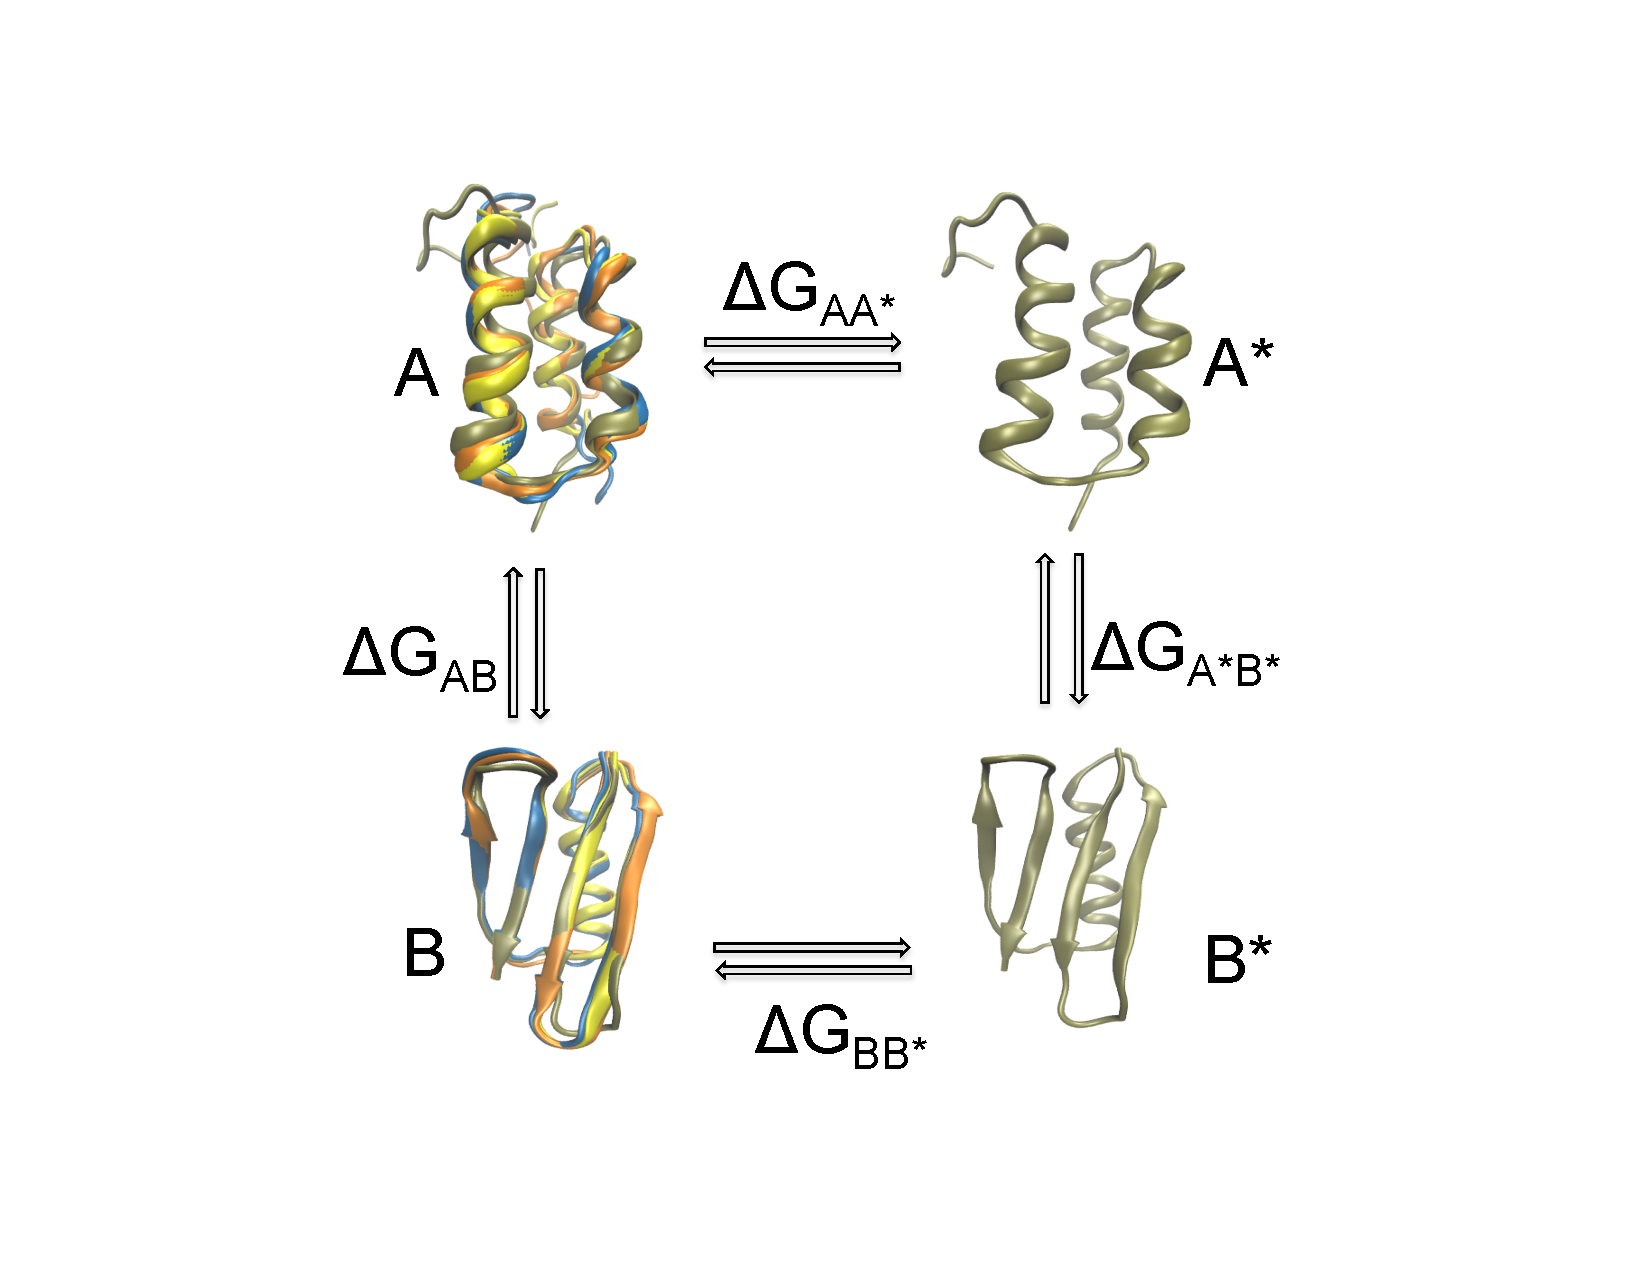
\includegraphics[width=14cm,height=14cm]{method.pdf}
\end{center}
\caption{Graphical representation of the thermodynamic cycle involving confinement method.}
\label{fig:method}
\end{figure}


\begin{figure}
\begin{center}
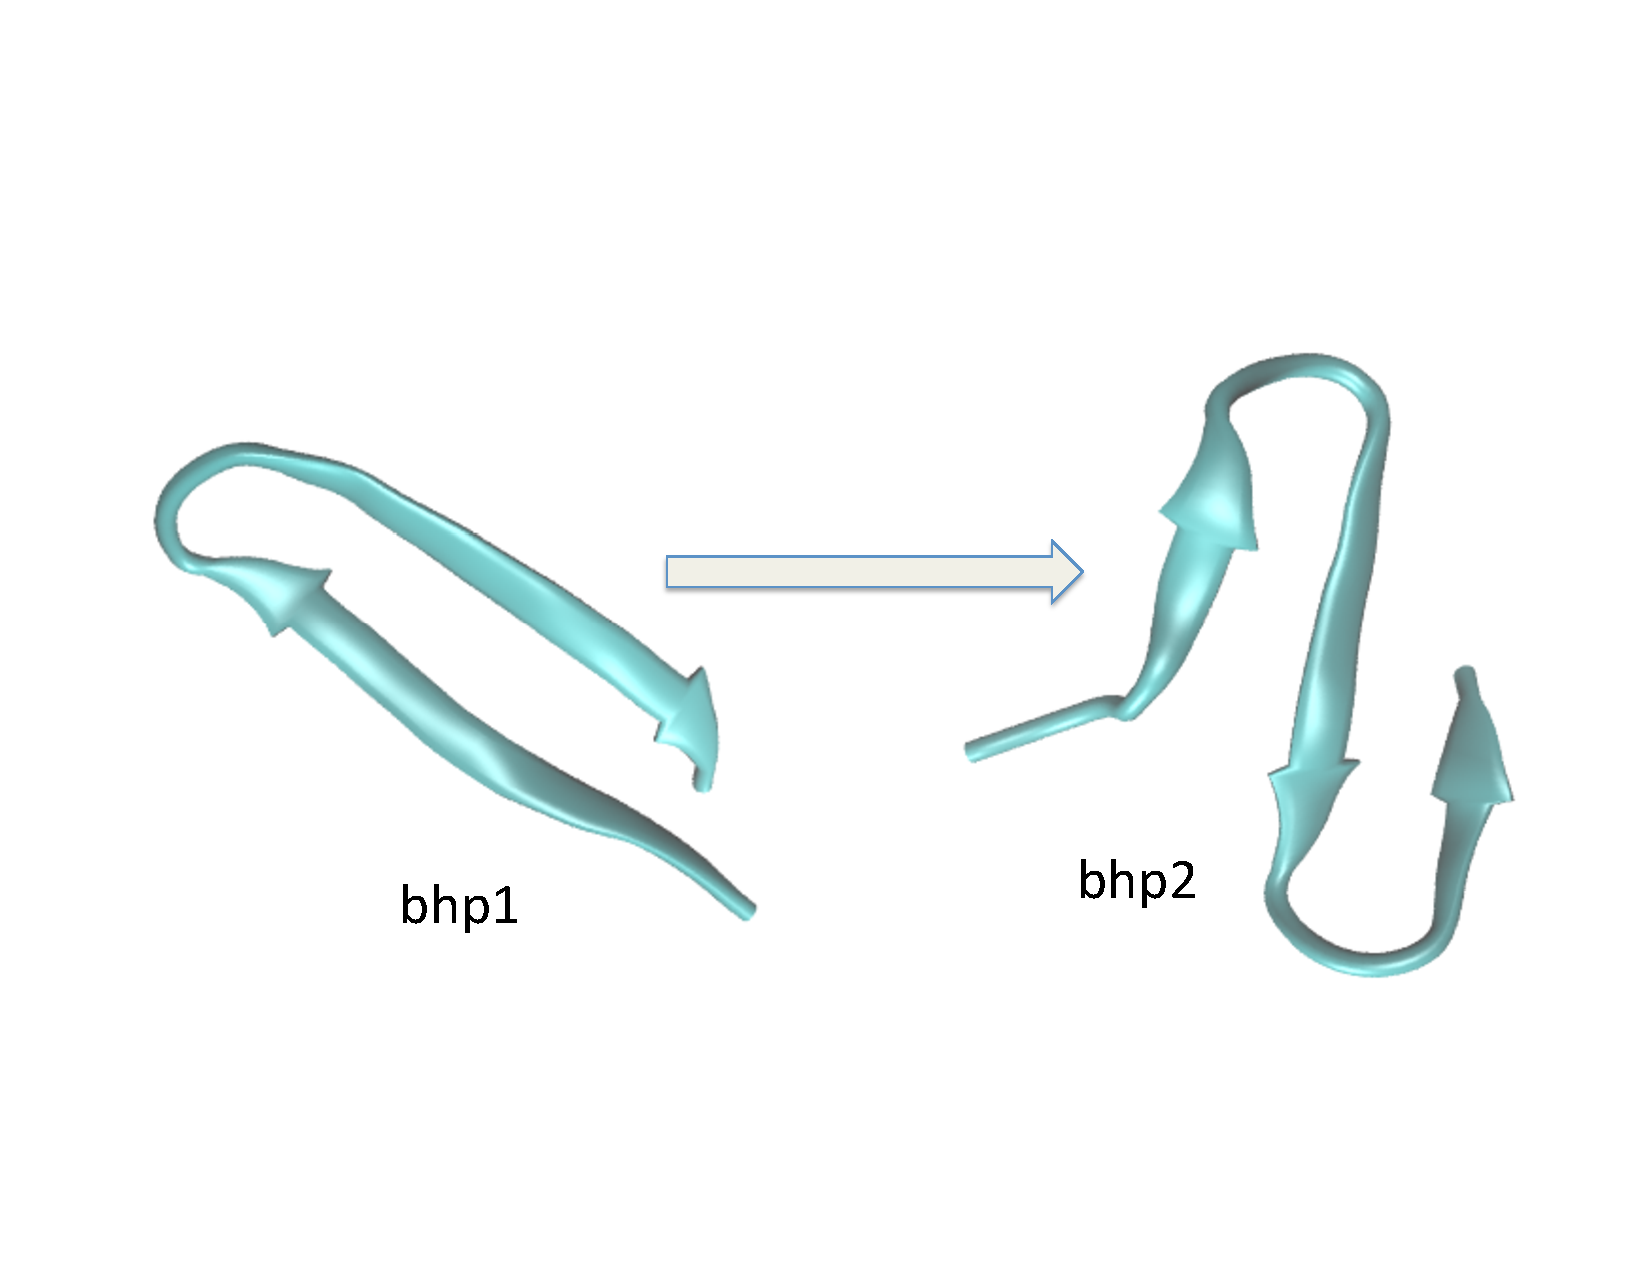
\includegraphics[width=12cm,height=10cm]{bhp.pdf}
\end{center}
\caption{Two conformations from $\beta$ hairpin from protein G, bhp1 and bhp2. The two stranded $\beta$ sheet, bhp1 is the native structure and the three stranded $\beta$ sheet is known as bhp3.}
\label{fig:bhp_conf}
\end{figure}

\begin{figure}
\begin{center}
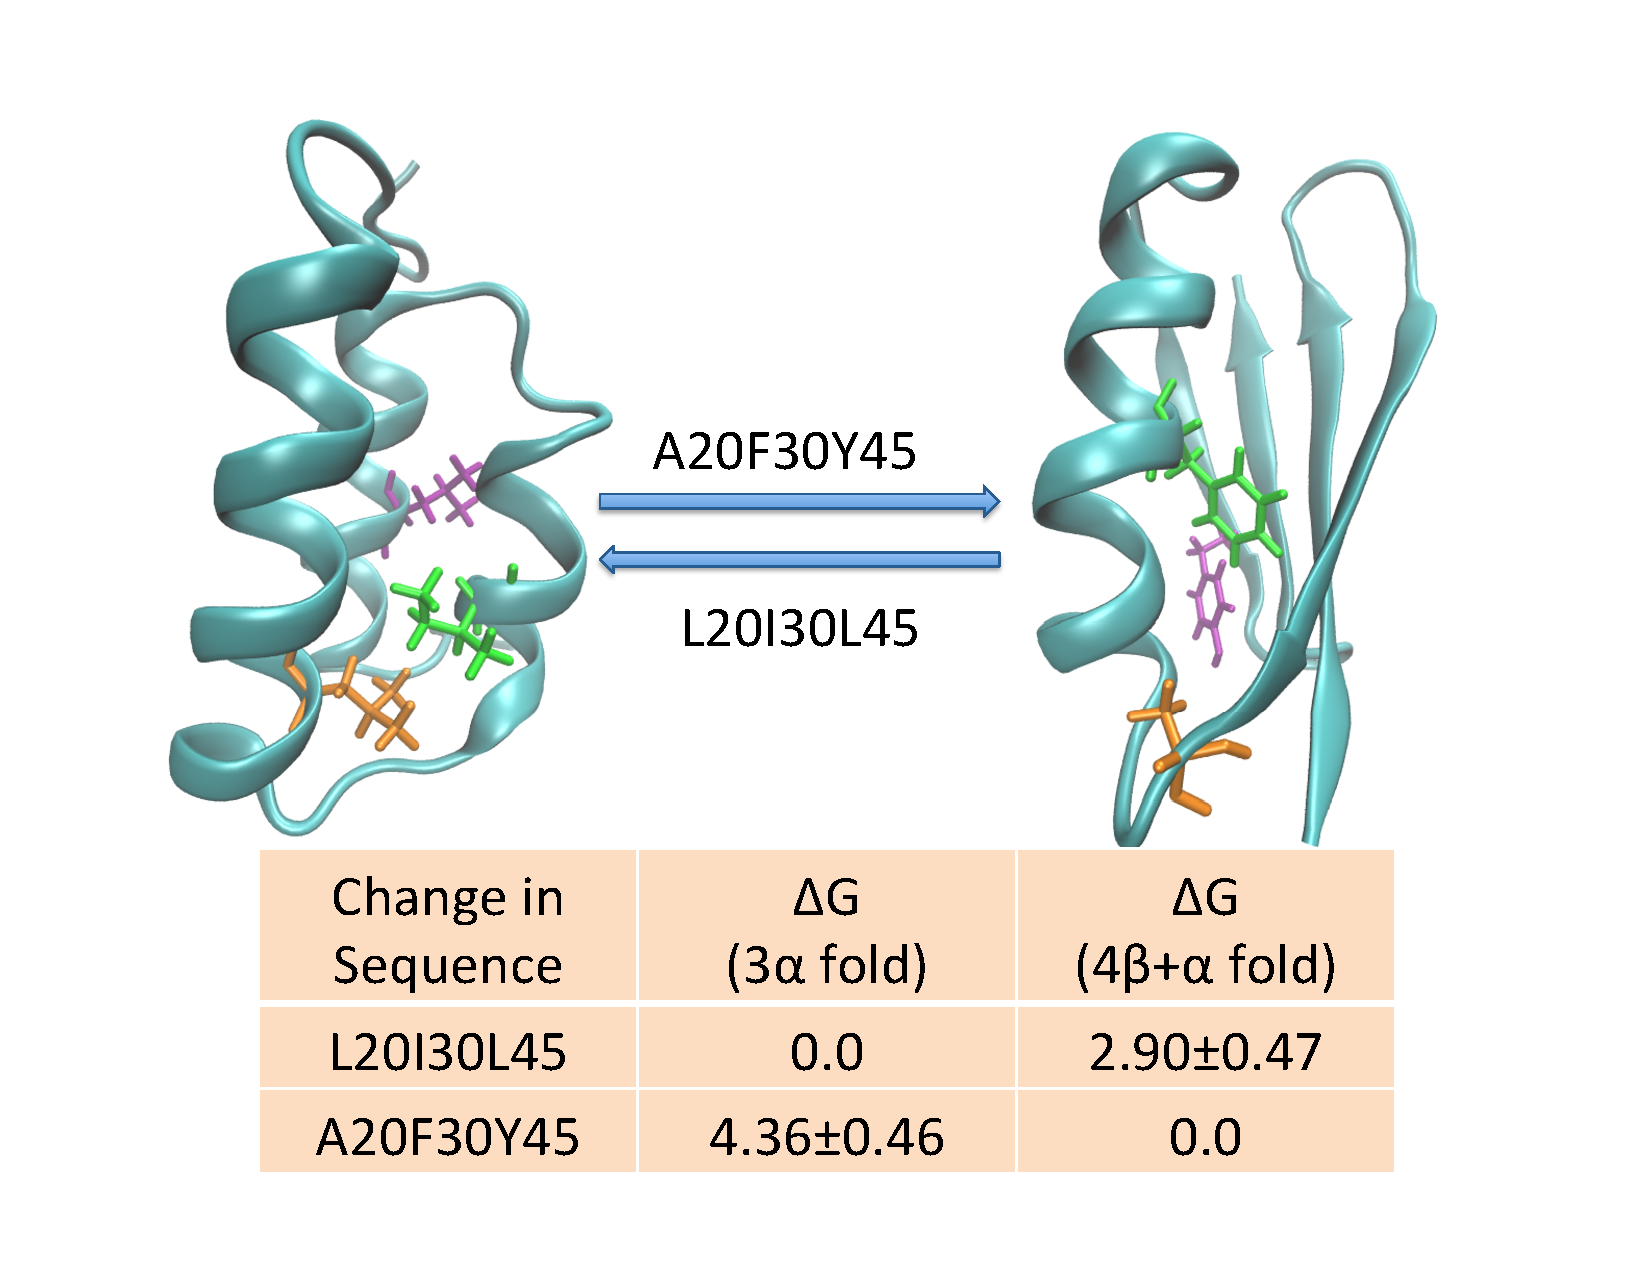
\includegraphics[width=12cm,height=10cm]{G95.pdf}
\end{center}
\caption{Two protein with 95 \% similar sequence but different folds}
\label{fig:G95}
\end{figure}

\begin{figure}
\begin{center}
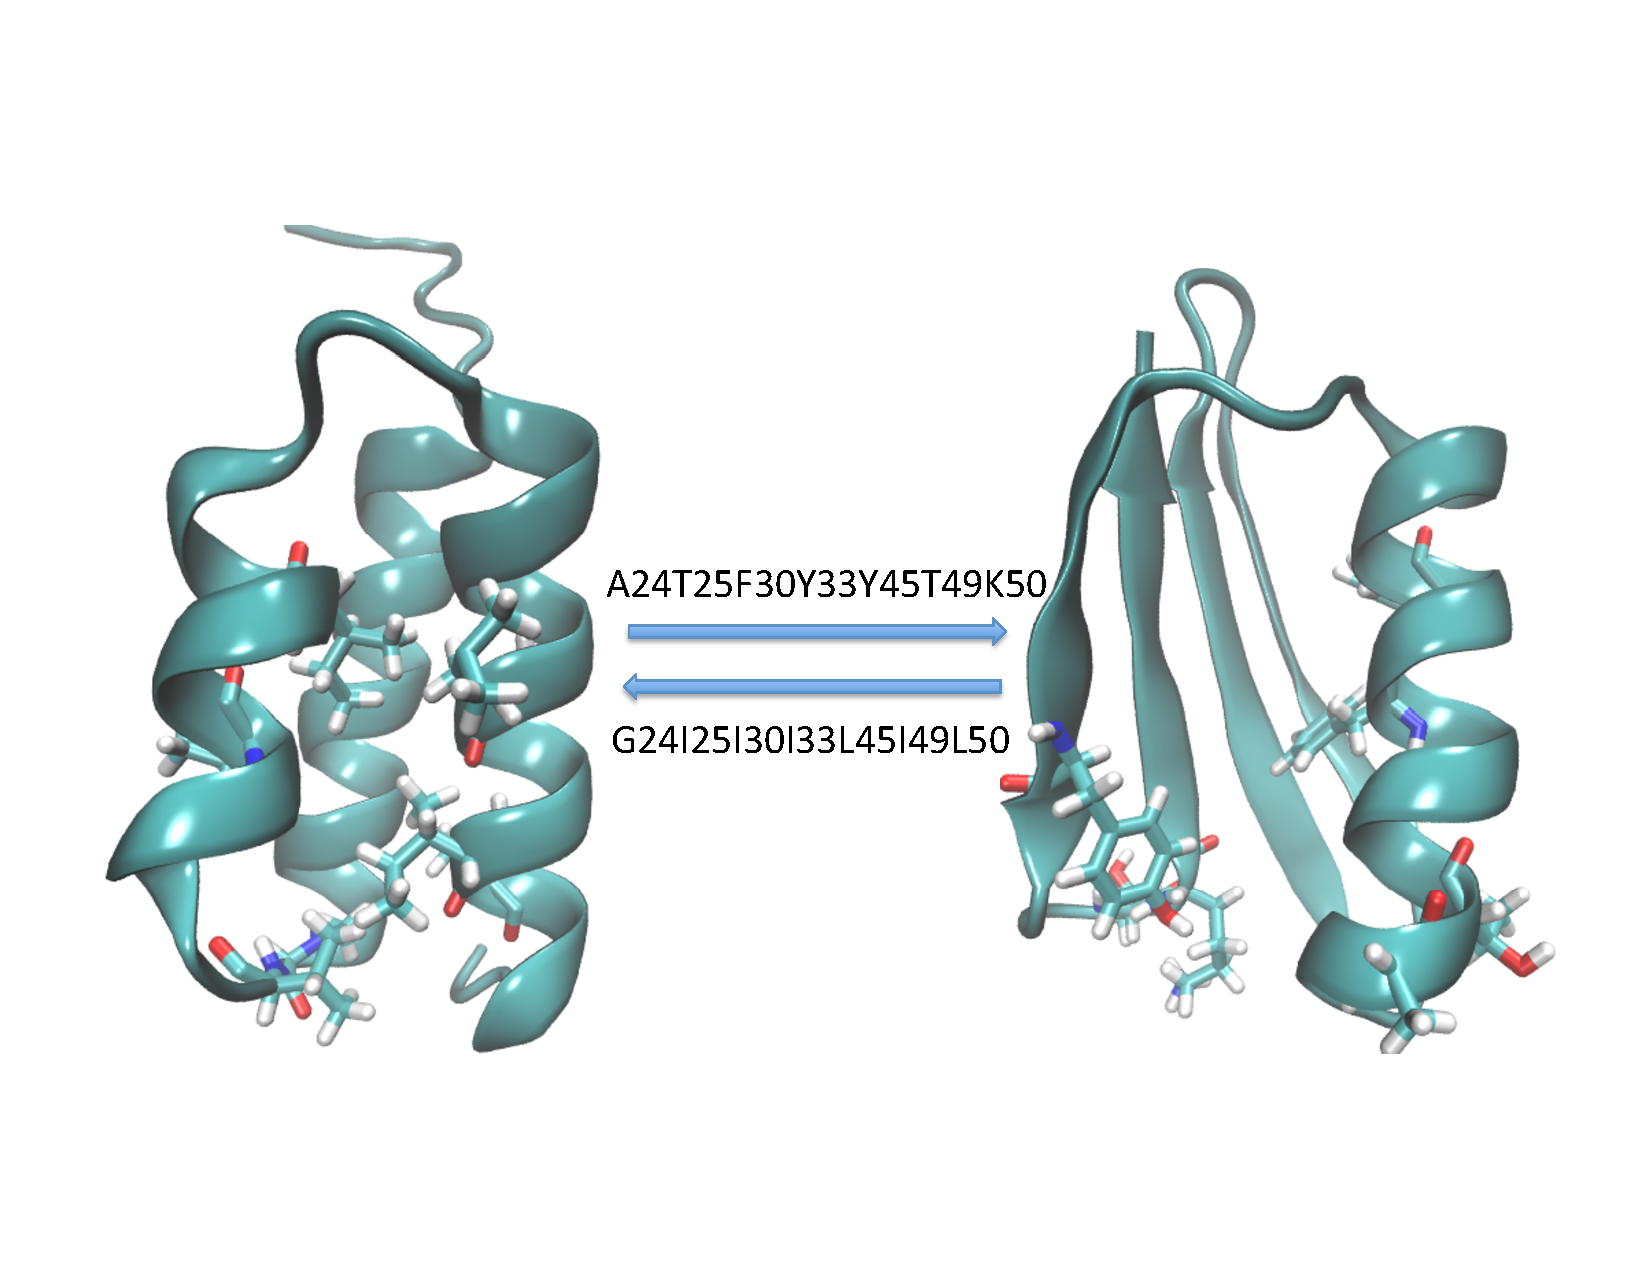
\includegraphics[width=12cm,height=10cm]{G88.pdf}
\end{center}
\caption{Two protein with 88 \% similar sequence but different folds}
\label{fig:G88}
\end{figure}

\begin{figure}
\begin{center}
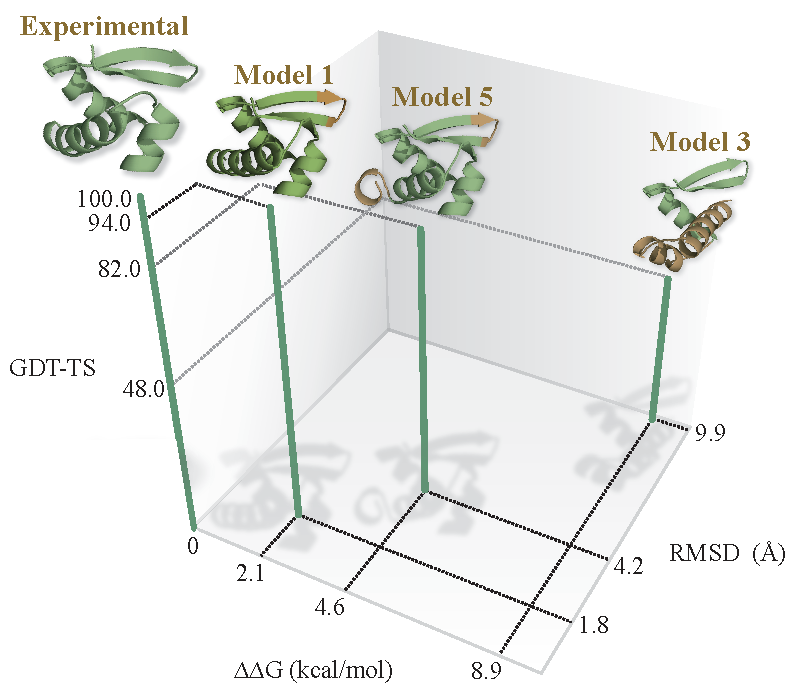
\includegraphics[width=12cm,height=10cm]{T0559.pdf}
\end{center}
\caption{Target T0559 from CASP9}
\label{fig:T0559}
\end{figure}

\begin{table}
\caption{The value of free energy and GDT\_TS for the CASP9 target T0559}
\label{tab:T0559}
\begin{center}
\begin{tabular}{l l l}\hline
Model   &     $\Delta G$ (Kcal/Mol) &  GDT\_TS \\ \hline
Model 1 &     0.000            &  94.03    \\
Model 3 &     $14.484 \pm 0.633$ &  48.13    \\
Model 5 &     $4.526  \pm 0.384$ &  82.46    \\ \hline
\end{tabular}
\end{center}
\end{table}

\begin{figure}
\begin{center}
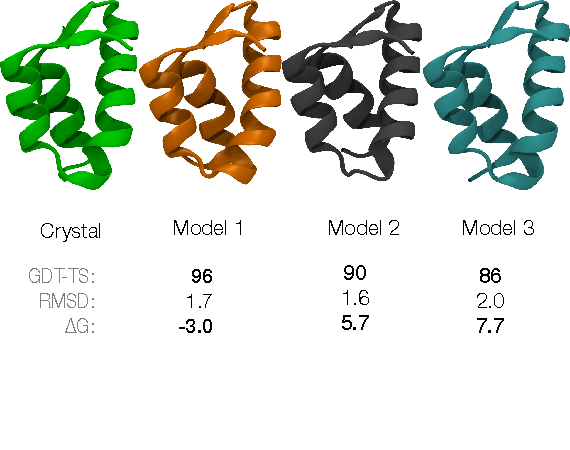
\includegraphics[width=12cm,height=10cm]{T0538.pdf}
\end{center}
\caption{Target T0538}
\label{fig:T0538}
\end{figure}

\begin{table}
\caption{The Free energy and GDT\_TS values of the CASP9 Target T0538}
\label{tab:T0538}
\begin{center}
\begin{tabular}{l l l l}\hline
Model   &     $\Delta G$ (Kcal/Mol) &  GDT\_TS & Group Submitted \\ \hline
Model 1 &     0.000              &  96.23    & PconsR  \\
Model 2 &     $15.891 \pm 0.475$ &  90.09  & Shell  \\
Model 3 &     $23.243 \pm 0.393$ &  86.32  & FOLDIT  \\
Model 4 &     $26.002 \pm 0.756$ &  80.66  & BAKER-ROSETTASERVER \\ \hline
\end{tabular}
\end{center}
\end{table}

\begin{figure}
\begin{center}
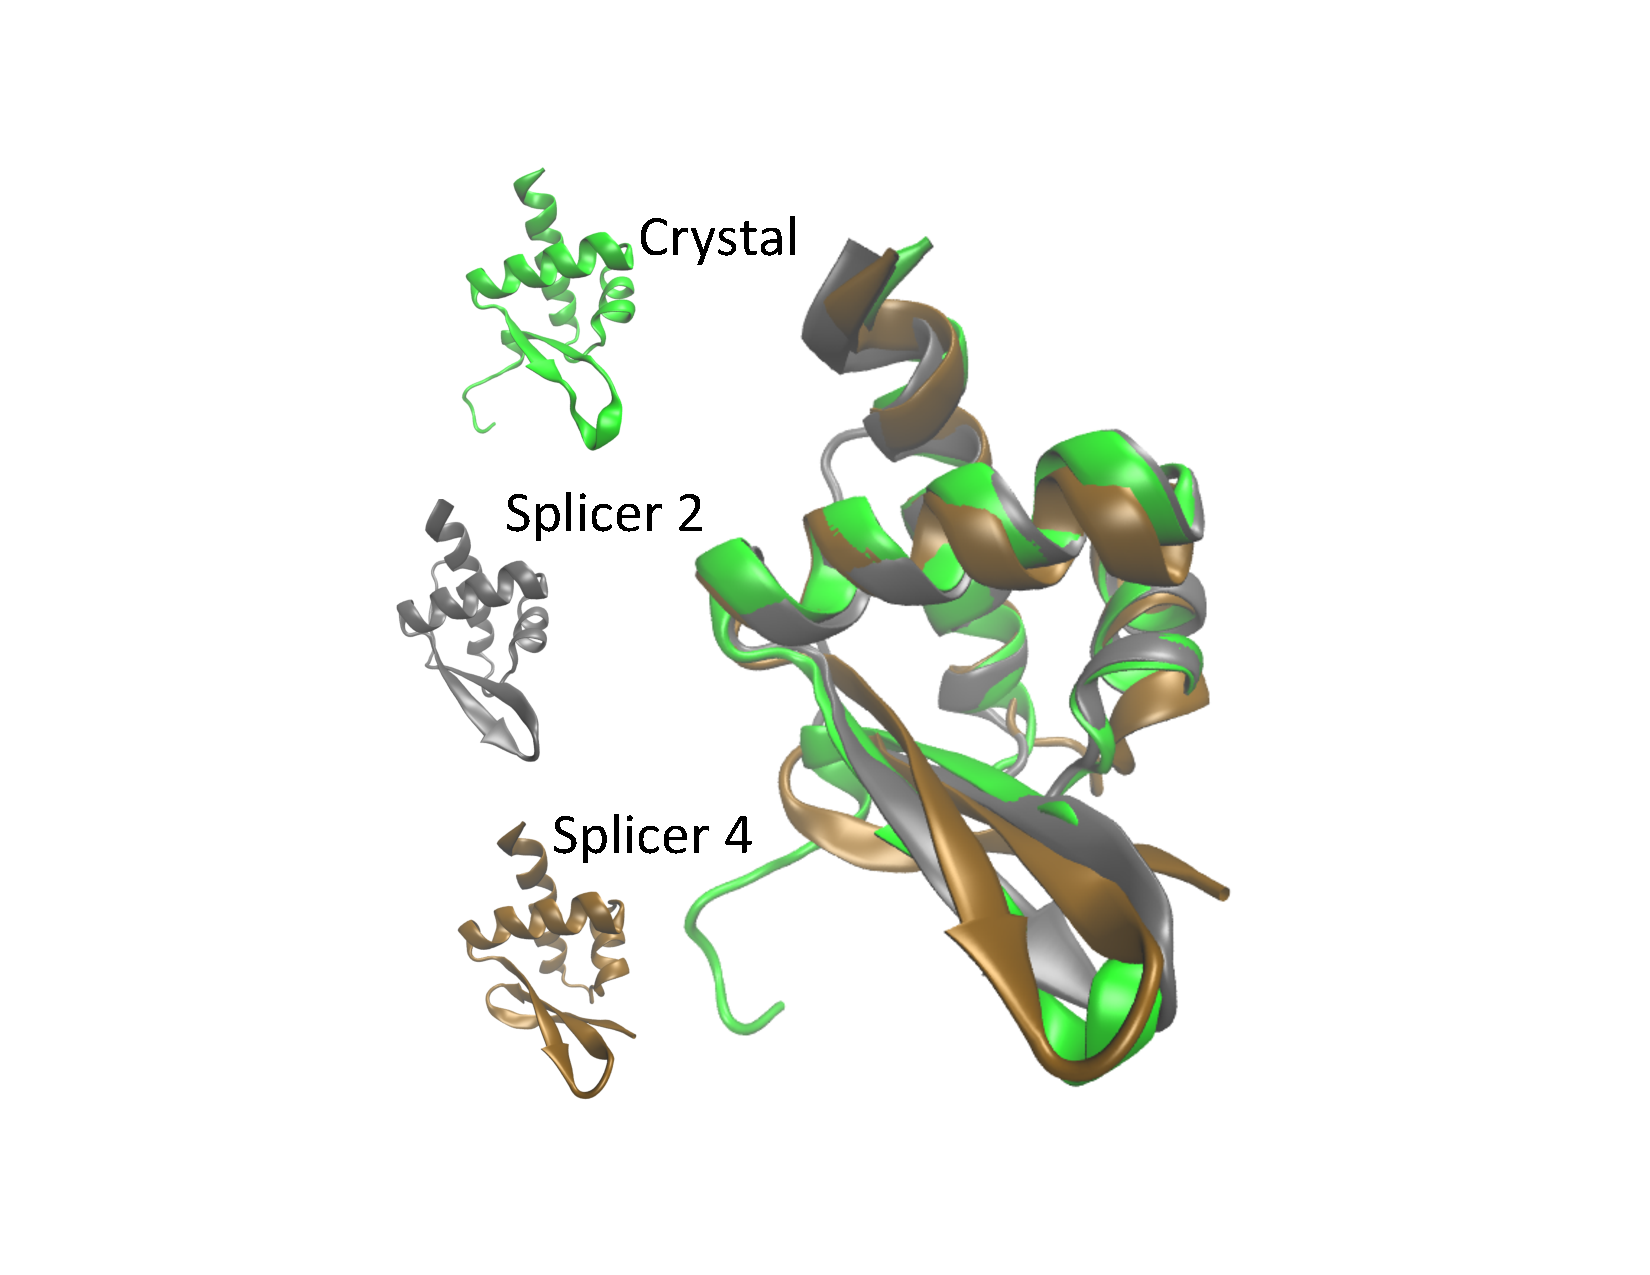
\includegraphics[width=12cm,height=10cm]{T0560.pdf}
\end{center}
\caption{Target T0560}
\label{fig:T0560}
\end{figure}

\begin{table}
\caption{The free energy and the GDT\_TS value of the CASP9 target T0560.}
\label{tab:T0560}
\begin{center}
\begin{tabular}{l l l}\hline
Model   &     $\Delta G$ (Kcal/Mol) &  GDT\_TS \\ \hline
Crystal &     0.000              & 100.00    \\
Model 2 &     $22.153 \pm 0.491$ &  94.14    \\
Model 4 &     $27.428  \pm 0.477$ &  76.56    \\ \hline
\end{tabular}
\end{center}
\end{table}


\begin{figure}
\begin{center}
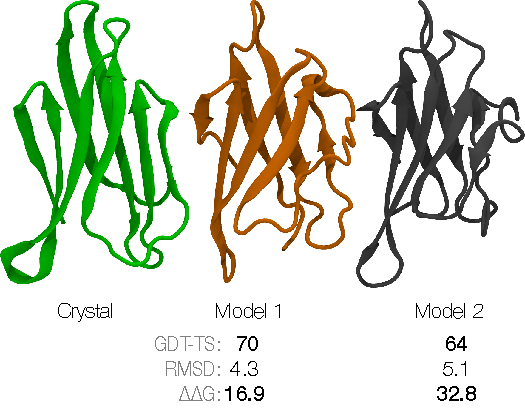
\includegraphics[width=12cm,height=10cm]{T0540.pdf}
\end{center}
\caption{T0540}
\label{fig:}
\end{figure}

\begin{table}
\caption{The free energy and the GDT\_TS value of the CASP9 target T0540.}
\label{tab:T0540}
\begin{center}
\begin{tabular}{l l l l}\hline
Model   &     $\Delta G$ (Kcal/Mol) &  GDT\_TS & Group Submitted \\ \hline
Crystal &     0.000              &  100.00   & -      \\
Model 1 &     $22.003 \pm 0.575$ &  69.72    & LTB    \\
Model 2 &     $53.786 \pm 0.553$ &  63.89    & Mufold \\ \hline
\end{tabular}
\end{center}
\end{table}

\begin{figure}
\begin{center}
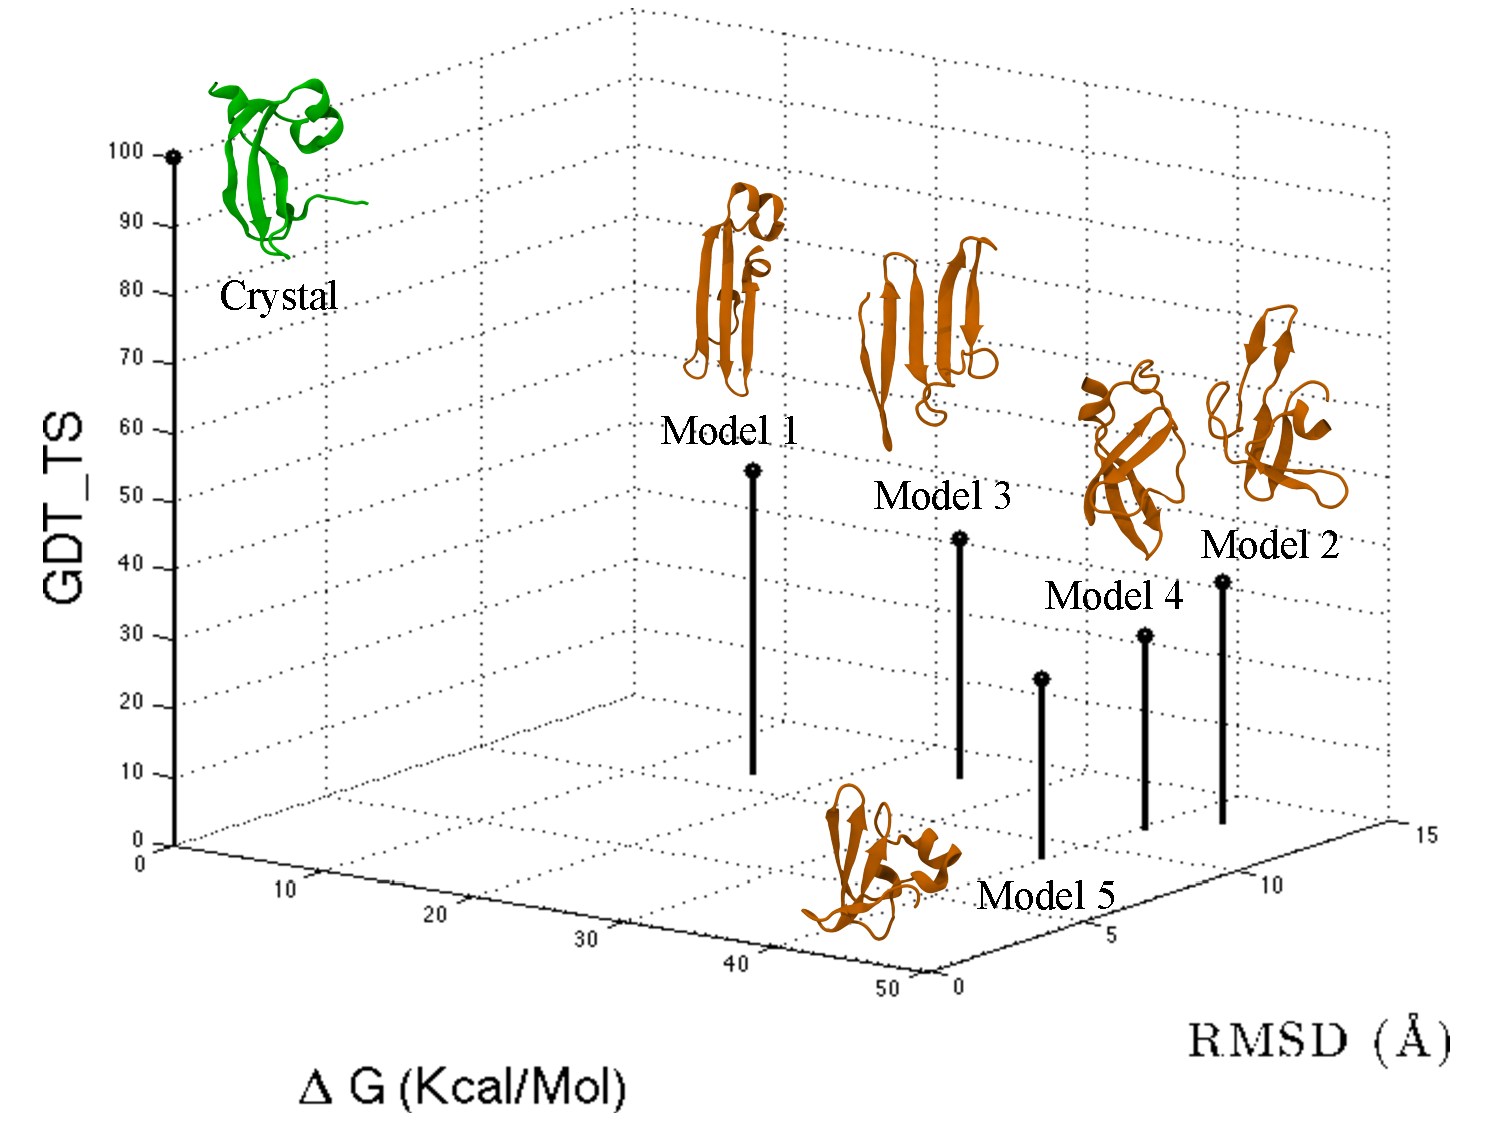
\includegraphics[width=12cm,height=10cm]{T0531.pdf}
\end{center}
\caption{T0531}
\label{fig:T0531}
\end{figure}

\begin{table}
\caption{The free energy and the GDT\_TS value of the CASP9 target T0531.}
\label{tab:T0531}
\begin{center}
\begin{tabular}{l l l}\hline
Model   &     $\Delta G$ (Kcal/Mol) &  GDT\_TS \\ \hline
Crystal &     0.000              & 100.00    \\
Model 1 &     $12.496 \pm 0.704$ &  43.53    \\
Model 2 &     $27.374 \pm 0.691$ &  34.48    \\
Model 3 &     $13.914 \pm 0.673$ &  34.48    \\
Model 4 &     $53.055 \pm 0.684$ &  28.02    \\
Model 5 &     $29.508 \pm 0.698$ &  25.86   \\ \hline
\end{tabular}
\end{center}
\end{table}

\begin{figure}
\begin{center}
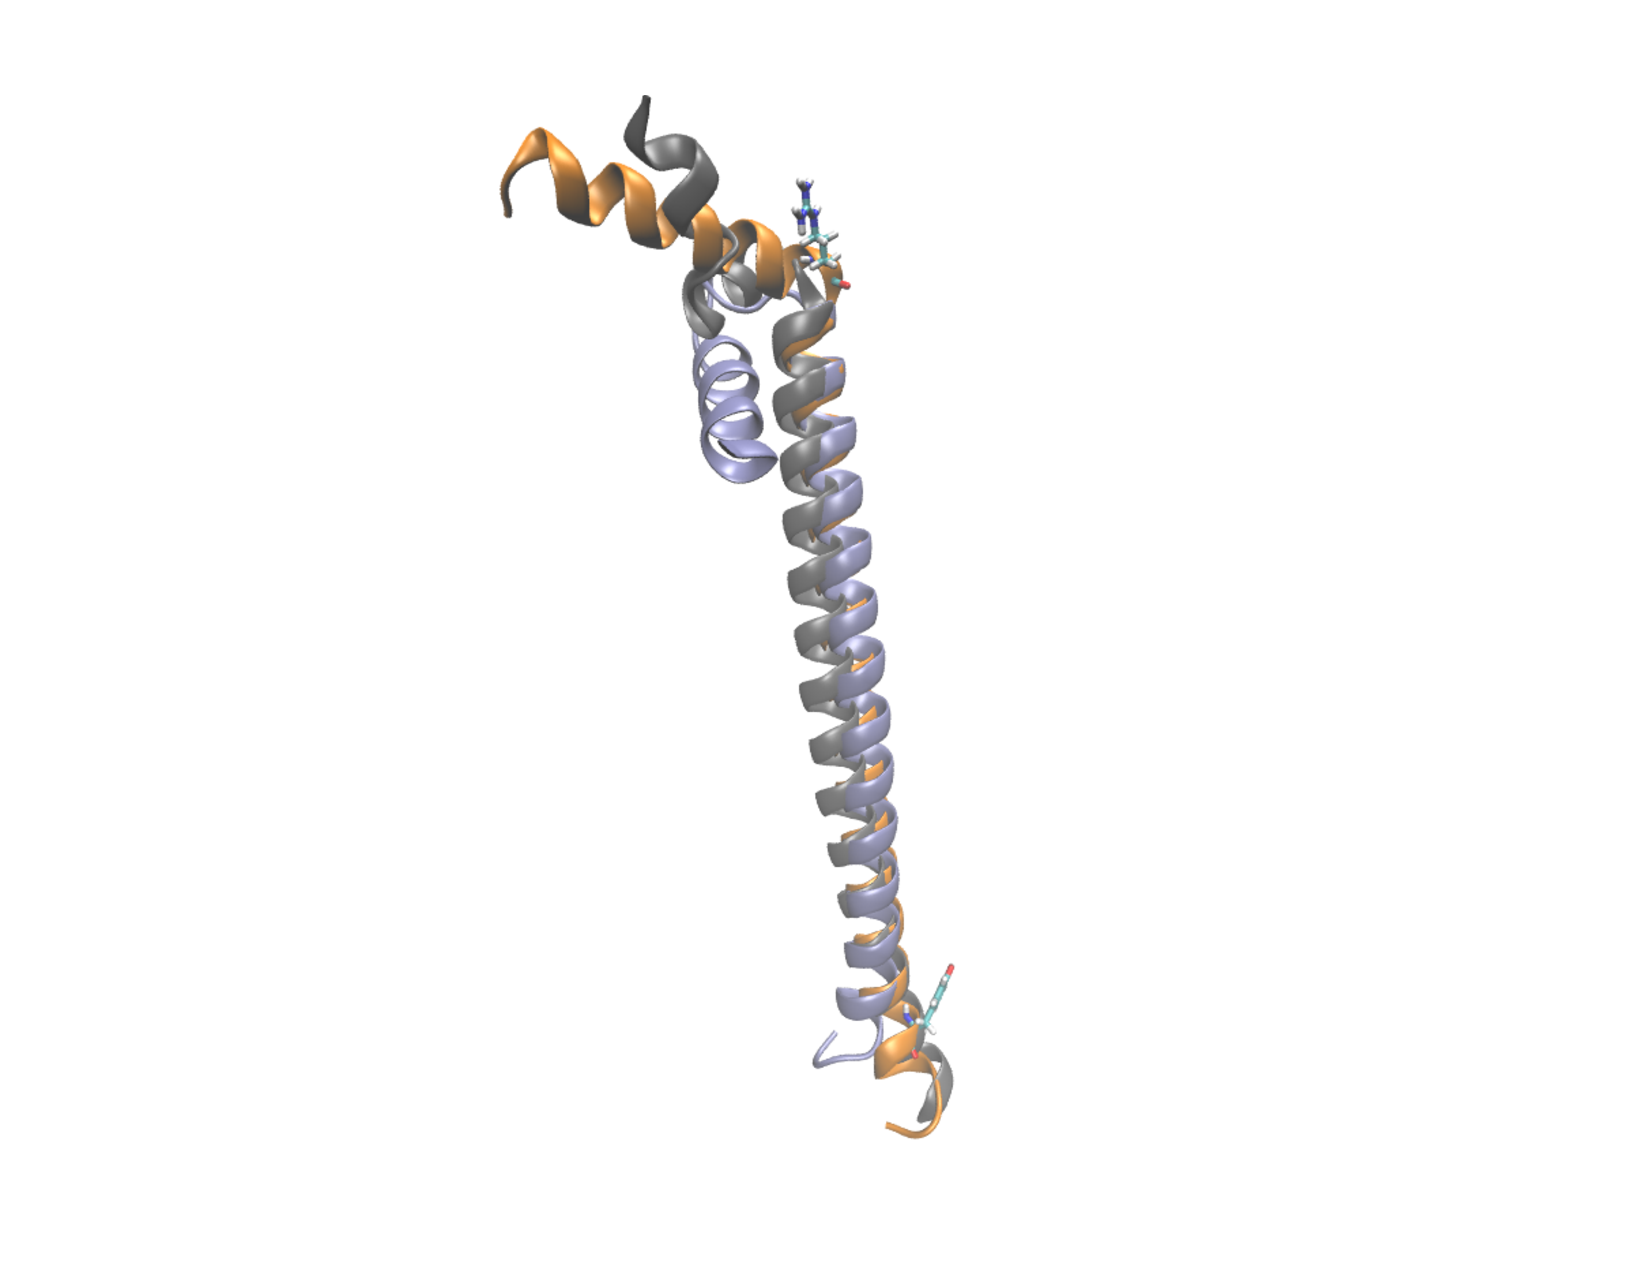
\includegraphics[width=12cm,height=10cm]{T0605.pdf}
\end{center}
\caption{T0605}
\label{fig:T0605}
\end{figure}


\begin{table}
\caption{The free energy and the GDT\_TS value of the CASP9 target T0605.}
\label{tab:T0605}
\begin{center}
\begin{tabular}{l l l}\hline
Model   &     $\Delta G$ (Kcal/Mol) &  GDT\_TS \\ \hline
Model 1 &     $0.000$ &  $97.96$    \\
Model 2 &     $1.689 \pm ?$ &  $89.29$    \\
Model 5 &     $16.064 \pm ?$ & $93.88$   \\ \hline
\end{tabular}
\end{center}
\end{table}



\section{Conclusion}



\section{Method}

The confinement method has been described in details in ref. by Tyka et.al. and Cecchini et. al.
Here we briefly describe the methodology.  We compute free energy $\Delta G_{AB}$ between A and B
conformation of the protein. For this purpose we use a thermodynamic cycle.

\begin{enumerate}

\item  We minimized both the conformation. These minimized conformation(A* and B*) are the
    restrained conformation of that state

\item Backbone dihedral angle of the whole protein is restrained by a harmonic potential to define
    the configurational state.

\item  In order to calculate the free energy $\Delta G_{A,A*}$ and  $\Delta G_{B,B*}$ A and B are
    gradually transformed in A* and B* by applying a harmonic restraint potential to all atom. For
    this purpose around 21 simulation were run each of 20 ns with increasing harmonic restraint
    potential from 0.00005 to 81.92 untill the free and the restrained state overlap well. The final
    restrained state was chosen so high so that the rotational contributional of the protein frozen
    out and only remaining contribution remain that of vibrational free enrgy. The fluctuation from
    the reference structure was recorded and the free energy is calculated using a numerical
    approach developed by Tyka et. al.

\item  Finally the thermodynamic cycle is closed by calculating the free energy between the final
    restrained state using normal mode analysis.

\end{enumerate}

In all the calculation amber 10 program is used with ff99SB with GB/SA implicit solvent.


\bibliographystyle{achemso}
\bibliography{paper}

Ytreberg, F.; Zuckerman, D. Simple estimation of absolute free energies for biomolecules. J. Chem. Phys. 2006, 124, 104105.

Park, S.; Lau, A.; Roux, B. Computing conformational free energy by deactivated morphing. J. Chem. Phys. 2008, 129, 134102

Zheng, L.; Chen, M.; Yang, W. Random walk in orthogonal space to achieve efficient free-energy simulation of complex systems, Proc. Natl. Acad. Sci. 2008, 105 (51), 20227.

Tyka, M.; Clarke, A.; Sessions, R. An Efficient, Path-Independent Method for Free-Energy Calculations. J.Phys.Chem. B 2006, 110, 17212–17220.


\end{document}

